\documentclass[../fem.tex]{subfile}

\begin{document}
\section{Solving Linear Systems of Equations}%
\label{sec:solving_linear_systems_of_equations}

A second major issue arises with the time complexity of computing the solution
to systems of linear equations. Trivial methods require $\O(n^3)$ time when
scaled to the magnitude of the matrices constructed, the time requirement
would become unacceptable. Thus we will examine a number of methods that can be
utilized in order to approximation the solution to systems of linear equations.

\subsection{Stationary Iterative Methods}%
\label{sub:stationary_iterative_methods}

All iterative methods can be expressed in the form
\begin{align*}
  x^{(k)}=Bx^{(k-1)}+c,
\end{align*}
when $B$ nor $c$ are dependent on the iteration $k$, then this is a stationary
iterative method. We comment on two stationary iterative methods
\textit{Jacobi}, and \textit{Gauss-Seidel} methods. There are several other
stationary iterative methods, but we limit ourselves to examining only these two
methods.

\subsubsection{Jacobi Method}%
\label{ssub:jacobi_method}

The Jacobi method is a very simple method for solving linear systems. It is
very easy to understand and implement, but the convergence of the approximation
can be very slow.

\begin{figure}[htpb]
  \centering
  \begin{tikzpicture}[scale=0.8]
\begin{axis}[axis lines=middle, xmin=10, xmax=500, ymin=0.000955884, ymax=3.85774,
x label style={at={(axis description cs:0.5,-0.1)},anchor=north},
y label style={at={(axis description cs:-0.15,.5)},rotate=90,anchor=south},
xlabel={$N$},
ylabel={$time(s)$} ]
\addplot[forget plot]
table{%
10 0.000955884
20 0.00209352
30 0.00321499
40 0.00481162
50 0.00570138
60 0.0110037
70 0.0145087
80 0.0211348
90 0.0292312
100 0.042789
110 0.0485071
120 0.0713184
130 0.101163
140 0.106837
150 0.126659
160 0.146752
170 0.174422
180 0.210044
190 0.244952
200 0.286659
210 0.31899
220 0.368238
230 0.418625
240 0.46899
250 0.536743
260 0.607371
270 0.677715
280 0.727596
290 0.791592
300 0.896709
310 0.978367
320 1.07977
330 1.1668
340 1.24879
350 1.39499
360 1.49532
370 1.63592
380 1.7198
390 1.85502
400 2.02816
410 2.16014
420 2.3453
430 2.48127
440 2.64986
450 2.88204
460 3.07034
470 3.27733
480 3.38639
490 3.61758
500 3.85774
};
\end{axis}
\end{tikzpicture}

  \caption{Time complexity of Jacobi method.}
  \label{fig:j_time}
\end{figure}

The concept for the Jacobi method is to solve for each variable $x_i$ one at a
time, with the assumption that all other variables are constant. We solve each
equation in isolation, and then the iteration provides us with our method for
converging to the actual solution. We consider the $i$he equation in the
system,
\begin{align*}
  \sum_{j=1}^na_{i,j}x_j=b_i.
\end{align*}
We then solve for the value of $x_i$ assuming all other values of $x$ are
fixed. We determine that
\begin{align*}
  x_i=\frac{b_i-\sum_{j\neq i}a_{i,j}x_j}{a_{i,i}}.
\end{align*}
We then implement the iteration to find the equation
\begin{align*}
  x_i^{(k)}=\frac{b_i-\sum_{j\neq i}a_{i,j}x_j^{(k-1)}}{a_{i,i}}.
\end{align*}

\begin{figure}[htpb]
  \centering
  \begin{tikzpicture}[scale=0.8]
\begin{axis}[axis lines=middle, xmin=10, xmax=500, ymin=6.90549e-15, ymax=3.37029e-12,
x label style={at={(axis description cs:0.5,-0.1)},anchor=north},
y label style={at={(axis description cs:-0.15,.5)},rotate=90,anchor=south},
xlabel={$N$},
ylabel={$error$}]
\addplot[forget plot]
table{%
10 3.37029e-12
20 7.92047e-13
30 3.04396e-13
40 1.0427e-13
50 3.65184e-13
60 1.09668e-13
70 9.3596e-14
80 7.2305e-14
90 1.43045e-13
100 2.25591e-14
110 7.02978e-14
120 1.767e-14
130 8.96556e-14
140 1.38426e-14
150 1.29263e-14
160 8.0989e-15
170 8.6539e-15
180 1.45368e-14
190 1.71589e-14
200 1.46895e-14
210 1.02967e-14
220 1.17107e-14
230 1.34722e-14
240 9.46449e-15
250 1.40114e-14
260 1.11627e-14
270 9.4128e-15
280 1.10491e-14
290 6.90549e-15
300 1.27176e-14
310 9.22616e-15
320 1.19022e-14
330 1.03847e-14
340 9.58546e-15
350 9.97699e-15
360 9.02912e-15
370 1.3828e-14
380 8.74999e-15
390 8.36753e-15
400 1.19304e-14
410 1.02126e-14
420 1.01072e-14
430 8.0742e-15
440 9.77824e-15
450 1.02938e-14
460 9.10134e-15
470 9.16966e-15
480 9.42344e-15
490 9.70977e-15
500 8.96426e-15
};
\end{axis}
\end{tikzpicture}

  \caption{Error of Jacobi method.}
  \label{fig:j_err}
\end{figure}

Using this formula for the computation of the new approximation vector $x$

\begin{algorithm}[H]
  \caption{Jacobi Method}\label{algo:jacobi_method}
  \begin{algorithmic}
    \State{$x=0$}
    \For{$k=1,2,\ldots$}
    \State{$\bar{x}=0$}
    \For{$i=1,2,\ldots,n$}
    \For{$j=1,2,\ldots,i-1,i+1,\ldots,n$}
    \State{$\wb{x}_i \pluseq a_{i,j}x_j$}
    \EndFor
    \State{$\bar{x}_i=\frac{b_i-\bar{x}_i}{a_{i,i}}$}
    \EndFor
    \State{$x=\bar{x}$}
    \If{$\Vert Ax-b\Vert\leq10^{-10}$}
    \State{\Return $x$}
    \EndIf
    \EndFor
    \State{\Return $x$}
  \end{algorithmic}
\end{algorithm}

Pseudocode for the Jacobi method is shown in Algorithm \ref{algo:jacobi_method}.
Note the necessity for a temporary $\bar{x}$ term, as the values of $x$ are
needed for the computation of the next iteration. We stop the iteration either
when a maximum iteration count is reached, or when our approximation is within
$10^{-10}$ of the actual solution. It is possible to alter this tolerance to
achieve either more precise approximation or to accelerate convergence at the
cost of accuracy.


\subsubsection{Gauss-Seidel Method}%
\label{ssub:gauss_seidel_method}

The Gauss-Seidel method is an extension of the Jacobi method, with one
optimization. Instead of using the old values of $x$, the algorithm uses the
already computed values of the current iteration.

\begin{figure}[htpb]
  \centering
  \begin{tikzpicture}[scale=0.8]
\begin{axis}[axis lines=middle, xmin=10, xmax=500, ymin=0.00044127, ymax=2.45767,
x label style={at={(axis description cs:0.5,-0.1)},anchor=north},
y label style={at={(axis description cs:-0.15,.5)},rotate=90,anchor=south},
xlabel={$N$},
ylabel={$time(s)$} ]
\addplot[forget plot]
table{%
10 0.00044127
20 0.000830058
30 0.00158482
40 0.0022026
50 0.00389241
60 0.00622612
70 0.00871826
80 0.0127367
90 0.0177076
100 0.0261929
110 0.0287522
120 0.0382489
130 0.0491408
140 0.0581017
150 0.0729747
160 0.085434
170 0.0984842
180 0.120965
190 0.156345
200 0.179699
210 0.208521
220 0.212536
230 0.268736
240 0.29001
250 0.341332
260 0.370696
270 0.413067
280 0.463962
290 0.514527
300 0.580587
310 0.615806
320 0.716396
330 0.743458
340 0.807671
350 0.882183
360 0.932908
370 1.02455
380 1.08536
390 1.18546
400 1.27366
410 1.41653
420 1.51655
430 1.56997
440 1.70138
450 1.82564
460 1.94822
470 2.05505
480 2.17154
490 2.30426
500 2.45767
};
\end{axis}
\end{tikzpicture}

  \caption{Time complexity of Gauss-Seidel method.}
  \label{fig:gs_time}
\end{figure}

This method does not improve the rate of convergence significantly, but it is a
simple to implement improvement over the Jacobi method. The mathematics and the
pseudocode are almost identical to that of the Jacobi method, with the only
difference being that instead of using $\bar{x}$ all values are taken from $x$.

\begin{figure}[htpb]
  \centering
  \begin{tikzpicture}[scale=0.8]
\begin{axis}[axis lines=middle, xmin=10, xmax=500, ymin=5.08708e-16, ymax=1.67915e-12,
x label style={at={(axis description cs:0.5,-0.1)},anchor=north},
y label style={at={(axis description cs:-0.15,.5)},rotate=90,anchor=south},
xlabel={$N$},
ylabel={$error$}]
\addplot[forget plot]
table{%
10 2.47488e-13
20 1.67915e-12
30 8.42348e-13
40 6.8434e-14
50 2.68464e-14
60 9.03398e-14
70 2.77213e-14
80 1.22813e-14
90 3.07682e-14
100 3.59455e-14
110 2.18452e-14
120 9.27237e-14
130 3.36351e-14
140 5.34724e-14
150 7.95896e-14
160 2.98958e-14
170 3.0989e-14
180 6.132e-14
190 7.97462e-16
200 7.80466e-16
210 6.5372e-16
220 5.17628e-14
230 7.83112e-16
240 4.04679e-14
250 7.77569e-16
260 6.42448e-16
270 6.22656e-16
280 6.62058e-16
290 5.08708e-16
300 6.79161e-16
310 6.50373e-16
320 7.06731e-16
330 6.97705e-16
340 7.06926e-16
350 6.96028e-16
360 6.045e-16
370 7.11762e-16
380 6.83487e-16
390 6.36232e-16
400 7.19029e-16
410 7.56739e-16
420 7.28104e-16
430 6.32255e-16
440 7.93183e-16
450 7.24263e-16
460 5.79839e-16
470 8.0121e-16
480 6.75056e-16
490 7.40416e-16
500 7.14274e-16
};
\end{axis}
\end{tikzpicture}

  \caption{Error of Gauss-Seidel method.}
  \label{fig:gs_err}
\end{figure}

Because of this similarity, we do not explain in detail the mathematics, but the
pseudocode is provided in Algorithm \ref{algo:gauss_seidel_method}.

\begin{algorithm}[H]
  \caption{Gauss-Seidel Method}\label{algo:gauss_seidel_method}
  \begin{algorithmic}
    \State{$x=0$}
    \For{$k=1,2,\ldots$}
    \For{$i=1,2,\ldots,n$}
    \State{$x_i=0$}
    \For{$j=1,2,\ldots,i-1,i+1,\ldots,n$}
    \State{$x_i \pluseq a_{i,j}x_j$}
    \EndFor
    \State{$x_i=\frac{b_i-x_i}{a_{i,i}}$}
    \EndFor
    \If{$\Vert Ax-b\Vert\leq10^{-10}$}
    \State{\Return $x$}
    \EndIf
    \EndFor
    \State{\Return $x$}
  \end{algorithmic}
\end{algorithm}

\subsection{Nonstationary Iterative Methods}%
\label{sub:nonstationary_iterative_methods}

Nonstationary methods differ from their stationary counterparts because the
computation involves information that is altered for every iteration. E.g. the
values of $B$ and $c$ can depend on the iteration count $k$. We discuss the
nonstationary iterative method called the  \textit{Conjugate Gradient} method.
All of the nonstationary iterative methods utilize Krylov subspaces, with the
exception of a few which we do not discuss.

\subsubsection{Conjugate Gradient Method}%
\label{ssub:conjugate_gradient_method}

This method is extremely effective for symmetric positive definite systems, and
it is one of the most researched nonstationary methods. This method is based on
the construction of a sequence of approximations. Each new approximation is
generated based on the direction required to minimize the residual.

\begin{figure}[htpb]
  \centering
  \begin{tikzpicture}[scale=0.8]
\begin{axis}[axis lines=middle, xmin=10, xmax=500, ymin=0.000121239,
ymax=1.69394,
x label style={at={(axis description cs:0.5,-0.1)},anchor=north},
y label style={at={(axis description cs:-0.15,.5)},rotate=90,anchor=south},
xlabel={$N$},
ylabel={$time(s)$} ]
\addplot[forget plot]
table{%
10 0.000121239
10.000000 0.000121
20 0.000604065
20.000000 0.000604
30 0.00164634
30.000000 0.001646
40 0.00283509
40.000000 0.002835
50 0.00277102
50.000000 0.002771
60 0.00467427
60.000000 0.004674
70 0.00733977
70.000000 0.007340
80 0.00981754
80.000000 0.009818
90 0.0141642
90.000000 0.014164
100 0.0180353
100.000000 0.018035
110 0.0220448
110.000000 0.022045
120 0.0291203
120.000000 0.029120
130 0.036587
130.000000 0.036587
140 0.0434833
140.000000 0.043483
150 0.052954
150.000000 0.052954
160 0.0654166
160.000000 0.065417
170 0.0764859
170.000000 0.076486
180 0.0894879
180.000000 0.089488
190 0.102215
190.000000 0.102215
200 0.128915
200.000000 0.128915
210 0.139589
210.000000 0.139589
220 0.157458
220.000000 0.157458
230 0.179333
230.000000 0.179333
240 0.199423
240.000000 0.199423
250 0.225927
250.000000 0.225927
260 0.253787
260.000000 0.253787
270 0.280379
270.000000 0.280379
280 0.317131
280.000000 0.317131
290 0.345662
290.000000 0.345662
300 0.386103
300.000000 0.386103
310 0.422678
310.000000 0.422678
320 0.4579
320.000000 0.457900
330 0.504794
330.000000 0.504794
340 0.553466
340.000000 0.553466
350 0.590098
350.000000 0.590098
360 0.647777
360.000000 0.647777
370 0.718308
370.000000 0.718308
380 0.781497
380.000000 0.781497
390 0.832744
390.000000 0.832744
400 0.888307
400.000000 0.888307
410 0.953204
410.000000 0.953204
420 1.00422
420.000000 1.004219
430 1.10199
430.000000 1.101993
440 1.16883
440.000000 1.168831
450 1.23442
450.000000 1.234425
460 1.32542
460.000000 1.325421
470 1.42446
470.000000 1.424458
480 1.53705
480.000000 1.537053
490 1.61991
490.000000 1.619915
500 1.69394
500.000000 1.693940
};
\end{axis}
\end{tikzpicture}

  \caption{Time complexity of Conjugate Gradient}
  \label{fig:cg_time}
\end{figure}

This is done by determining which ``direction'' must be used in order to
minimize the residual, then the approximation is moved by some $\alpha$ amount
in that direction. After repeating this process for some number of iterations,
the generated approximation should be converging to the actual solution.

\begin{figure}[htpb]
  \centering
     \begin{tikzpicture}[scale=0.8]
\begin{axis}[axis lines=middle, xmin=10, xmax=500, ymin=3.36449e-14, ymax=7.46005e-12,
x label style={at={(axis description cs:0.5,-0.1)},anchor=north},
y label style={at={(axis description cs:-0.15,.5)},rotate=90,anchor=south},
xlabel={$N$},
ylabel={$error$}]
\addplot[forget plot]
table{%
10 7.46005e-12
10.000000 0.000000
20 2.17131e-12
20.000000 0.000000
30 1.49511e-12
30.000000 0.000000
40 1.87031e-12
40.000000 0.000000
50 9.85293e-13
50.000000 0.000000
60 5.87844e-13
60.000000 0.000000
70 9.59211e-13
70.000000 0.000000
80 2.6936e-13
80.000000 0.000000
90 3.30694e-13
90.000000 0.000000
100 2.99461e-13
100.000000 0.000000
110 1.65521e-13
110.000000 0.000000
120 1.99588e-13
120.000000 0.000000
130 1.53808e-13
130.000000 0.000000
140 9.12794e-14
140.000000 0.000000
150 1.97419e-13
150.000000 0.000000
160 7.85794e-14
160.000000 0.000000
170 9.94596e-14
170.000000 0.000000
180 9.93811e-14
180.000000 0.000000
190 9.85562e-14
190.000000 0.000000
200 1.00703e-13
200.000000 0.000000
210 1.31656e-13
210.000000 0.000000
220 8.6859e-14
220.000000 0.000000
230 8.5972e-14
230.000000 0.000000
240 5.39787e-14
240.000000 0.000000
250 7.06746e-14
250.000000 0.000000
260 7.76623e-14
260.000000 0.000000
270 5.06525e-14
270.000000 0.000000
280 6.25117e-14
280.000000 0.000000
290 6.88223e-14
290.000000 0.000000
300 6.18314e-14
300.000000 0.000000
310 6.23921e-14
310.000000 0.000000
320 5.56555e-14
320.000000 0.000000
330 4.9641e-14
330.000000 0.000000
340 5.13226e-14
340.000000 0.000000
350 4.95898e-14
350.000000 0.000000
360 5.97346e-14
360.000000 0.000000
370 5.28114e-14
370.000000 0.000000
380 5.03734e-14
380.000000 0.000000
390 4.65883e-14
390.000000 0.000000
400 4.73715e-14
400.000000 0.000000
410 5.02019e-14
410.000000 0.000000
420 4.53782e-14
420.000000 0.000000
430 3.82739e-14
430.000000 0.000000
440 4.53222e-14
440.000000 0.000000
450 3.80655e-14
450.000000 0.000000
460 3.59027e-14
460.000000 0.000000
470 4.26115e-14
470.000000 0.000000
480 3.90466e-14
480.000000 0.000000
490 4.3247e-14
490.000000 0.000000
500 3.36449e-14
500.000000 0.000000
};
\end{axis}
\end{tikzpicture}

  \caption{Error of Conjugate Gradient}
  \label{fig:cg_err}
\end{figure}

We construct the iterative approximation in each iteration by a multiple of
$\alpha_i$ of the search direction $p^{(i)}$,
\begin{align*}
  x^{(i)}=x^{(i-1)}+\alpha_ip^{(i)}.
\end{align*}
We then update the residual $r^{(i)}=b-Ax^{(i)}$ as
\begin{align*}
  q^{(i)}&=Ap^{(i)}\\
  r^{(i)}&=r^{(i-1)}-\alpha_i q^{(i)}
\end{align*}
We construct $\alpha_i$ inorder to minimize ${r^{(i)}}^TA^{-1}r^{(i)}$,
\begin{align*}
  \alpha_i=\frac{{r^{(i-1)}}^Tr^{(i-1)}}{{p^{(i)}}^TAp^{(i)}}.
\end{align*}
Then to updated the search direcitons using the residual
\begin{align*}
  \beta_i&=\frac{{r^{(i)}}^Tr^{(i)}}{{r^{(i-1)}}^Tr^{(i-1)}}\\
  p^{(i)}&=r^{9)}+\beta_{i-1}p^{(i-1)}
\end{align*}
where the choice of $\beta_i$ ensures that $r^{(i)}$ and $r^{(i-1)}$ are
orthogonal.

This process ties together the construction of the Krylov subspace, and the
construction of the approximation based off of the most recently computed
krylov basis vector. This means that if we allow our iterations to proceed
until $N$ iterations, then we should have constructed the complete Krylov
subspace, and thus our approximation should be exact.

Using this approximation we can construct our pseudocode of the algorithm. Which
is presented in Algorithm \ref{algo:conjugategradient}.

\begin{algorithm}[H]
  \caption{ConjugateGradient}\label{algo:conjugategradient}
  \begin{algorithmic}
    \State{$x=0$}
    \State{$r=b-Ax$}
    \For{$i=1,2,\ldots,n$}
    \State{$\rho^{(i)}={\Vert r \Vert}^2$}
    \If{$i=0$}
    \State{$p=r$}
    \Else
    \State{$\beta=\frac{\rho^{(i)}}{\rho^{(i-1)}}$}
    \State{$p=r$}
    \EndIf
    \State{$q=Ap$}
    \State{$\alpha=\frac{\rho^{(i)}}{\left<p,q\right>}$}
    \State{$x\pluseq \alpha p$}
    \State{$r\minuseq \alpha q$}
    \If{$\Vert r \Vert \leq 10^{-10}$}
    \State{\Return $x$}
    \EndIf
    \EndFor
    \State{\Return $x$}
  \end{algorithmic}
\end{algorithm}

\subsection{Cholesky Method}%
\label{sub:cholesky_method}

The Cholesky method is a method for solving systems of linear equations based
upon the Cholesky decomposition of a matrix. This is the only direct method
that we consider. A direct method does not depend on the convergence of a sequence,
but instead directly solves the system of equations. This method is useful for
the purpose of time prediction. The convergence of iterative methods greatly
depends on the system being considered, using this method the time required is
directly related to the number of elements. This means that each system of the
same size will require the same time to solve.

\begin{figure}[htpb]
  \centering
     \begin{tikzpicture}[scale=0.8]
\begin{axis}[axis lines=middle, xmin=10, xmax=500, ymin=9.9297e-05,
ymax=35.1002,
x label style={at={(axis description cs:0.5,-0.1)},anchor=north},
y label style={at={(axis description cs:-0.15,.5)},rotate=90,anchor=south},
xlabel={$N$},
ylabel={$time(s)$} ]
\addplot[forget plot]
table{%
10 9.9297e-05
10.000000 0.000099
20 0.000700153
20.000000 0.000700
30 0.00241376
30.000000 0.002414
40 0.00452465
40.000000 0.004525
50 0.00638056
50.000000 0.006381
60 0.0127957
60.000000 0.012796
70 0.0213059
70.000000 0.021306
80 0.0320726
80.000000 0.032073
90 0.0499284
90.000000 0.049928
100 0.0718767
100.000000 0.071877
110 0.102187
110.000000 0.102187
120 0.164281
120.000000 0.164281
130 0.188823
130.000000 0.188823
140 0.249047
140.000000 0.249047
150 0.323534
150.000000 0.323534
160 0.429071
160.000000 0.429071
170 0.521841
170.000000 0.521841
180 0.657483
180.000000 0.657483
190 0.795538
190.000000 0.795538
200 0.971675
200.000000 0.971675
210 1.18065
210.000000 1.180646
220 1.43207
220.000000 1.432070
230 1.66826
230.000000 1.668258
240 1.9756
240.000000 1.975603
250 2.31886
250.000000 2.318862
260 2.68266
260.000000 2.682664
270 3.11233
270.000000 3.112333
280 3.6044
280.000000 3.604404
290 4.10074
290.000000 4.100741
300 4.69147
300.000000 4.691466
310 5.36752
310.000000 5.367517
320 6.0468
320.000000 6.046796
330 6.85027
330.000000 6.850266
340 8.64613
340.000000 8.646129
350 8.61681
350.000000 8.616810
360 9.61479
360.000000 9.614794
370 10.6977
370.000000 10.697731
380 11.8896
380.000000 11.889554
390 13.1546
390.000000 13.154559
400 14.6085
400.000000 14.608493
410 16.0706
410.000000 16.070635
420 17.7679
420.000000 17.767872
430 19.3644
430.000000 19.364384
440 21.2335
440.000000 21.233512
450 23.1883
450.000000 23.188308
460 25.3093
460.000000 25.309303
470 27.5244
470.000000 27.524385
480 29.8963
480.000000 29.896318
490 32.3767
490.000000 32.376666
500 35.1002
500.000000 35.100232
};
\end{axis}
\end{tikzpicture}

  \caption{Time complexity of Cholesky method.}
  \label{fig:ch_time}
\end{figure}

The Cholesky decomposition of a matrix provides a lower triangular matrix $L$
of the form
\begin{align*}
  A=LL^T
\end{align*}

We use this decomposition of $A$ to solve two systems of linear equations,
using forward and back substitution, which is an efficient method for finding
these solutions.
\begin{align*}
  Ly&=b\quad\text{by forward substitution}\\
  L^Tx&=y\quad\text{by back substitution}.\\
\end{align*}
This provides the solution $x$ to the system of linear equations.

We present a plot of the time requirements for the computation in
Figure \ref{fig:ch_time}.

\subsubsection{Cholesky Decomposition}%
\label{ssub:cholesky_decomposition}


We utilize the Cholesky-Banachiewicz algorithm for the construction of the
lower triangular matrix $L$. This algorithm states that
\begin{align*}
  L_{j,j}&=\sqrt{A_{j,j}-\sum_{k=1}^{j-1}L_{j,k}^2}\\
  L_{i,j}&=\frac{1}{L_{j,j}}\left(A_{i,j}-\sum_{k=1}^{j-1}L_{i,k}L_{j,k}\right)\
  \text{for}\ i>j.
\end{align*}
This construction of the Cholesky decomposition is very easy, and fairly
efficient. Thus allowing us to preform this decomposition easily.

\subsubsection{Forward/Back Substitution}%
\label{ssub:forward_back_substitution}

The method of forward and back substitution is an efficient method for solving
systems of linear equations of the form $Lx=b$ where $L$ is a lower triangular
matrix. Note that the process is almost identical for an upper triangular
matrix, just with the order of iteration flipped. We will only provide an
explanation for forward substitution.

The first stage is to write the system of equations like so
\begin{align*}
  \begin{matrix}
    L_{1,1}x_1 & & & & =b_1\\
    L_{2,1}x_1 & +L_{2,2}x_2 & & & =b_2\\
    \vdots & \vdots & \ddots & & \vdots\\
    L_{n,1}x_1 & +L_{n,2}x_2 & \cdots & L_{n,n}x_n & =b_2\\
  \end{matrix}.
\end{align*}
We can clearly solve for $x_1$ directly, and find
\begin{align*}
  x_1=\frac{b_1}{L_{1,1}}.
\end{align*}

It is possible to substitute this into the second equation. This will cause the
second equation to only have one unknown $x_2$, and so we can directly solve
for $x_2$. This process is repeated for all $x$. Providing the general
expression
\begin{align*}
  x_m=\frac{b_m-\sum_{i=1}^{m-1}L_{m,i}x_i}{L_{m,m}}.
\end{align*}
This expression can then be used to compute the solution to the system of
linear equations.

Using the Cholesky decomposition and forward and back substitution, we are able
to compute the exact solution to the system of equations, without resorting the
inefficient Gaussian elimination.

We provide pseudocode of this method in Algorithm \ref{algo:cholesky_method}.

\begin{algorithm}[H]
  \caption{Cholesky method}\label{algo:cholesky_method}
  \begin{algorithmic}
    \State{}\Comment{Calculate $A=LL^T$ decomposition.}
    \For{$j=0,1,2,\ldots,N$}
    \State{$L_{j,j}=0$}
    \For{$k=0,1,2,\ldots,j$}
    \State{$L_{j,j}\pluseq L_{j,k}^2$}
    \EndFor
    \State{$L_{j,j}=\sqrt{A_{j,j}-L_{j,j}}$}
    \For{$i=j,j+1,j+2,\ldots,N$}
    \State{$L_{i,j}=0$}
    \For{$k=0,1,2,\ldots,j$}
    \State{$L_{i,j} \pluseq L_{i,k}L_{j,k}$}
    \EndFor
    \State{$L_{i,j}=\frac{A_{i,j}-L_{i,j}}{L_{j,j}}$}
    \EndFor
    \EndFor
    \State{}\Comment{Calculate $Ly=b$ by forward substitution.}
    \State{$y=0$}
    \For{$i=1,2,\ldots,N$}
    \State{$y_i=0$}
    \For{$j=1,2,\ldots,i$}
    \State{$y_i\pluseq L_{i,j}y_j$}
    \EndFor
    \State{$y_i=\frac{b_i-y_i}{L_{i,i}}$}
    \EndFor
    \State{}\Comment{Calculate $L^Tx=y$ by back substitution.}
    \State{$x=0$}
    \For{$i=N,N-1,\ldots,1$}
    \State{$x_i=0$}
    \For{$j=i+1,i+2,\dots,N$}
    \State{$x_i\pluseq L^T_{i,j}x_j$}
    \EndFor
    \State{$x_i=\frac{b_i-x_i}{L^T_{i,i}}$}
    \EndFor
    \State{\Return $x$}
  \end{algorithmic}
\end{algorithm}

\subsection{Issues}%
\label{sub:issues}

We note that these algorithms have requirements on the form of the matrix $A$.
For many of these, the algorithm requires a symmetric positive definite matrix.
We comment on some of these restrictions here.

We note that future work must be done to determine if the global matrix that is
constructed by the Finite Element Method will consistently satisfy these
restraints. If it does then it is possible to provide extra optimizations based
on the form of the global matrix. If a general form of the matrix cannot be
guaranteed, then we will be forced to utilize significantly slower methods of
computing the solution to the linear system.

\begin{figure}[htpb]
  \centering
   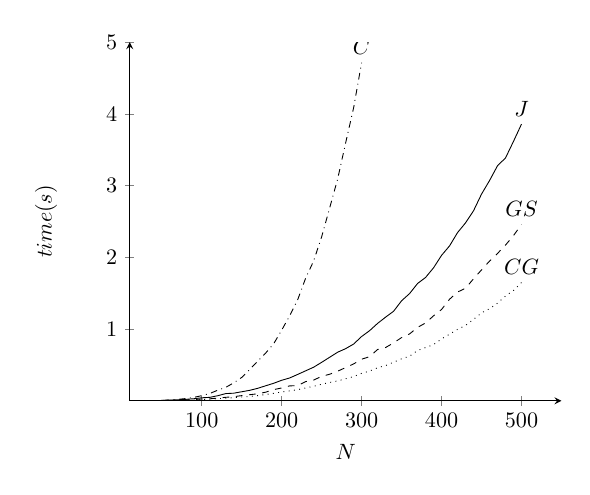
\begin{tikzpicture}[scale=0.8]
\definecolor{color0}{RGB}{0,0,0}
\begin{axis}[axis lines=middle, xmin=10, xmax=550, ymin=0.000171516, ymax=5,
x label style={at={(axis description cs:0.5,-0.1)},anchor=north},
y label style={at={(axis description cs:-0.15,.5)},rotate=90,anchor=south},
xlabel={$N$},
ylabel={$time(s)$} ]
\addplot[color0,  forget plot]
table{%
10 0.000955884
20 0.00209352
30 0.00321499
40 0.00481162
50 0.00570138
60 0.0110037
70 0.0145087
80 0.0211348
90 0.0292312
100 0.042789
110 0.0485071
120 0.0713184
130 0.101163
140 0.106837
150 0.126659
160 0.146752
170 0.174422
180 0.210044
190 0.244952
200 0.286659
210 0.31899
220 0.368238
230 0.418625
240 0.46899
250 0.536743
260 0.607371
270 0.677715
280 0.727596
290 0.791592
300 0.896709
310 0.978367
320 1.07977
330 1.1668
340 1.24879
350 1.39499
360 1.49532
370 1.63592
380 1.7198
390 1.85502
400 2.02816
410 2.16014
420 2.3453
430 2.48127
440 2.64986
450 2.88204
460 3.07034
470 3.27733
480 3.38639
490 3.61758
500 3.85774
} node[above] {$J$};
\addplot[color0, dashed, forget plot]
table{%
10 0.00044127
20 0.000830058
30 0.00158482
40 0.0022026
50 0.00389241
60 0.00622612
70 0.00871826
80 0.0127367
90 0.0177076
100 0.0261929
110 0.0287522
120 0.0382489
130 0.0491408
140 0.0581017
150 0.0729747
160 0.085434
170 0.0984842
180 0.120965
190 0.156345
200 0.179699
210 0.208521
220 0.212536
230 0.268736
240 0.29001
250 0.341332
260 0.370696
270 0.413067
280 0.463962
290 0.514527
300 0.580587
310 0.615806
320 0.716396
330 0.743458
340 0.807671
350 0.882183
360 0.932908
370 1.02455
380 1.08536
390 1.18546
400 1.27366
410 1.41653
420 1.51655
430 1.56997
440 1.70138
450 1.82564
460 1.94822
470 2.05505
480 2.17154
490 2.30426
500 2.45767
} node[above] {$GS$};
\addplot[color0, dotted, forget plot]
table{%
10 0.000601359
20 0.000952636
30 0.00137694
40 0.00175361
50 0.00293501
60 0.00568654
70 0.00675084
80 0.0094955
90 0.013371
100 0.0181317
110 0.0223123
120 0.0300225
130 0.0370952
140 0.044599
150 0.0540593
160 0.0618763
170 0.0731524
180 0.088562
190 0.105139
200 0.123779
210 0.139108
220 0.156012
230 0.180335
240 0.202153
250 0.232086
260 0.256144
270 0.278185
280 0.30815
290 0.338558
300 0.383299
310 0.415675
320 0.461685
330 0.49211
340 0.538913
350 0.585691
360 0.622517
370 0.701708
380 0.743409
390 0.78352
400 0.864041
410 0.928453
420 0.996619
430 1.05168
440 1.13663
450 1.22582
460 1.28518
470 1.36083
480 1.46231
490 1.53924
500 1.64908
} node[above] {$CG$};
\addplot[color0, dashdotted, forget plot]
table{%
10 0.000341451
20 0.00114773
30 0.00189575
40 0.00311467
50 0.00662719
60 0.0121988
70 0.020523
80 0.031794
90 0.0482962
100 0.0720558
110 0.102228
120 0.14824
130 0.187536
140 0.250288
150 0.32627
160 0.43764
170 0.552088
180 0.666092
190 0.795475
200 0.985347
210 1.1846
220 1.40866
230 1.71039
240 1.94972
250 2.28616
260 2.68764
270 3.09182
280 3.59459
290 4.08491
300 4.71359
} node[above] {$C$};
\end{axis}
\end{tikzpicture}

  \caption{Plots of the different time requirements for solvign the linear
  systems.}
  \label{fig:times}
\end{figure}

\subsubsection{Possitive Definite}%
\label{ssub:possitive_definite}

All of these algorithms require a positive definite matrix. This is required to
guarantee that there is a unique solution to the system. This can be considered
to ensure that there is a minimum in some $N$ dimensional space, instead of a
saddle, or maximum. Only with a minimum can we minimize our residual and use
gradient descent to find our equilibrium solution.

\subsubsection{Symmetric}%
\label{ssub:symmetric}

Most of these algorithms, with the exception of the Gauss-Seidel method,
require the matrix to be symmetric. This requirement is mostly for
computational efficiency and simplicity of the algorithm. There are some
methods that can be adapted to function for nonsymmetric matrices, but those
become significantly more complex. For our implementation we will be restricted
to the Gauss-Seidel method, as the matricies in the linear systems are not
symmetric. For better preformance, it is recommended to utilize the Generalized
Minimum Residual method, as this can handle non-symmetric matricies and is
significantly faster than Gauss-Seidel method.


\end{document}
